\chapter{Theoretical Background \label{chap:2_TheoreticalBackground}}

    %%%%%%%%%%%%%%%%%%
    % Grammarly: 100/100
    %%%%%%%%%%%%%%%%%%
    In this chapter, we present the background of the main concepts regarding our study. The focus is to present the main software components of an \acl{USV} (Section~\ref{sec:gnc_system}), and present the international regulations (\acs{COLREGS}) for navigation of vessels on water  (Section~\ref{sec:colregs}).

\section{GNC System}
\label{sec:gnc_system}    
    %%%%%%%%%%%%%%%%%%
    % Grammarly: 99/100
    %%%%%%%%%%%%%%%%%%
    
    \begin{figure}[H]
        \centering
        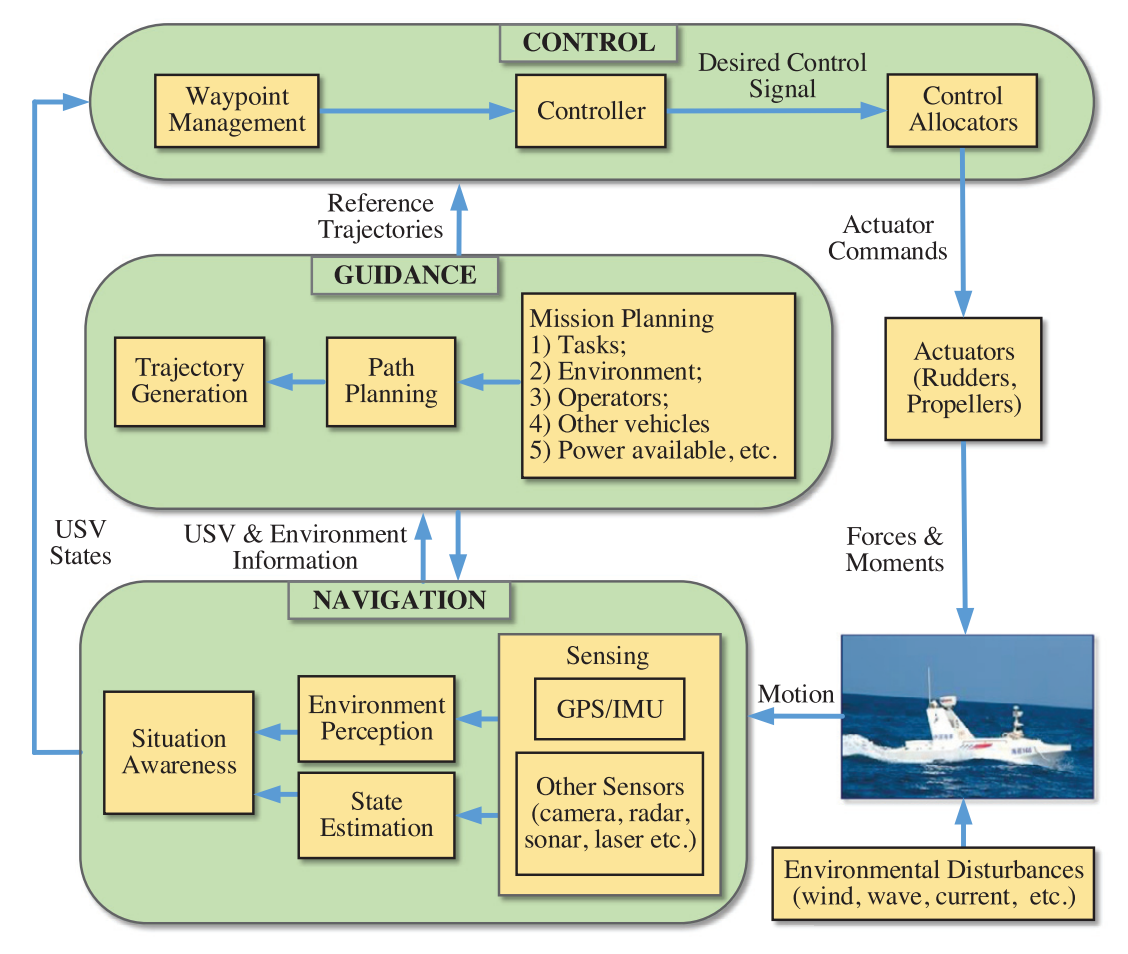
\includegraphics[scale=0.85]{figs/Chap2/Liu2016Unmanned_GNCSystem.png}
        \caption{\ac{GNC} System Modules~\cite{Liu2016Unmanned}}
        \label{fig:Liu2016Unmanned_GNCSystem}
    \end{figure}
    
    The \acs{GNC} system is an essential component for most \acp{USV}, being responsible for managing partially or entirely the \ac{USV}. \acs{GNC} stands for Guidance, Navigation, and Control. In this section, we describe the responsibilities of each one of the \ac{GNC} modules as well as the interaction between them. The Figure \ref{fig:Liu2016Unmanned_GNCSystem}, presented by Liu~\cite{Liu2016Unmanned}, summarizes the \acs{GNC} modules, their responsibilities, and interactions.
    
    %%%%%%%%%%%%%%%%%%
    % Grammarly: 100/100
    %%%%%%%%%%%%%%%%%%
    In short, the guidance system is responsible for the determination of the \ac{USV}'s trajectory to achieve a goal location. For trajectory generation, the guidance system uses the information provided by the navigation system regarding the environment (\eg~obstacles around and general disturbances such as wind and current) and related to the \ac{USV}'s state (\eg~current location). After generating the trajectory, the guidance system makes the route available to the control system. The control system generates actuation commands to change the \ac{USV}'s state and effectively move the \ac{USV}. We present detailed explanations about the \ac{GNC} modules in the following sections.
    
    \subsection{Guidance System}
    
    %%%%%%%%%%%%%%%%%%
    % Grammarly: 100/100
    %%%%%%%%%%%%%%%%%%
    In an autonomous approach, most \acp{USV} guidance systems are responsible for planning the path that will be traveled by the \ac{USV}. For the determination of a path, the guidance system uses the information gathered by the navigation system regarding the environment and the \ac{USV}'s state. In general, trajectory generation shall consider the \ac{USV} mission and marine protocols, such as being under the \ac{COLREGS} or respect \ac{TSS} definitions (\ac{TSS} are similar to traffic ground lines that must be respected by vessels on navigation at sea.) Also, information about vehicle capability (e.g., maximum speed and power consumption) and environmental conditions (e.g., wind, wave, and current disturbance) may be required to determine suitable trajectories.
    
    %%%%%%%%%%%%%%%%%%
    % Grammarly: 100/100
    %%%%%%%%%%%%%%%%%%
    Typical implementations of the guidance system propose the usage of global and local planners~\cite{Liu2016Unmanned}. The global planner is responsible for path planning related to the far-field based on well-known information about the environment, such as islands, coasts, bridges over water \etc, assuming a deliberative behavior. Conversely, the local planner is responsible for path planning regarding the near-field environment, assuming a reactive behavior when detecting other vessels or obstacles. Conventional methods for path planning applied to \ac{USV} guidance are based on heuristic search~\cite{Liu2016Unmanned}, such as A*~\cite{Larson2006Autonomous, Naus2013Idea}. Some works used optimization methods for \ac{USV}`s path planning but presented several limitations in real-world trials, due to expensive computational cost~\cite{Svec2011Trajectory, Campbell2013Automatic}.

    %%%%%%%%%%%%%%%%%%
    % Grammarly: 100/100
    %%%%%%%%%%%%%%%%%%
    In Figure \ref{fig:chap2_globallocalpath}, we illustrate the difference between global and local planning in our context. For a situation where our vessel (henceforth referred to as \ac{OV}) is not capable of detecting some vessel in the far-field, the global planner could define a route above a location occupied by an approaching vessel (henceforth referred to as \ac{AV}). In this situation, the local planner should react when an \ac{AV} appears in the near-field and define an avoidance behavior. Both global and local planners usually define the \ac{USV} trajectory considering static and dynamic obstacles.
    
    \begin{figure}[H]
        \centering
        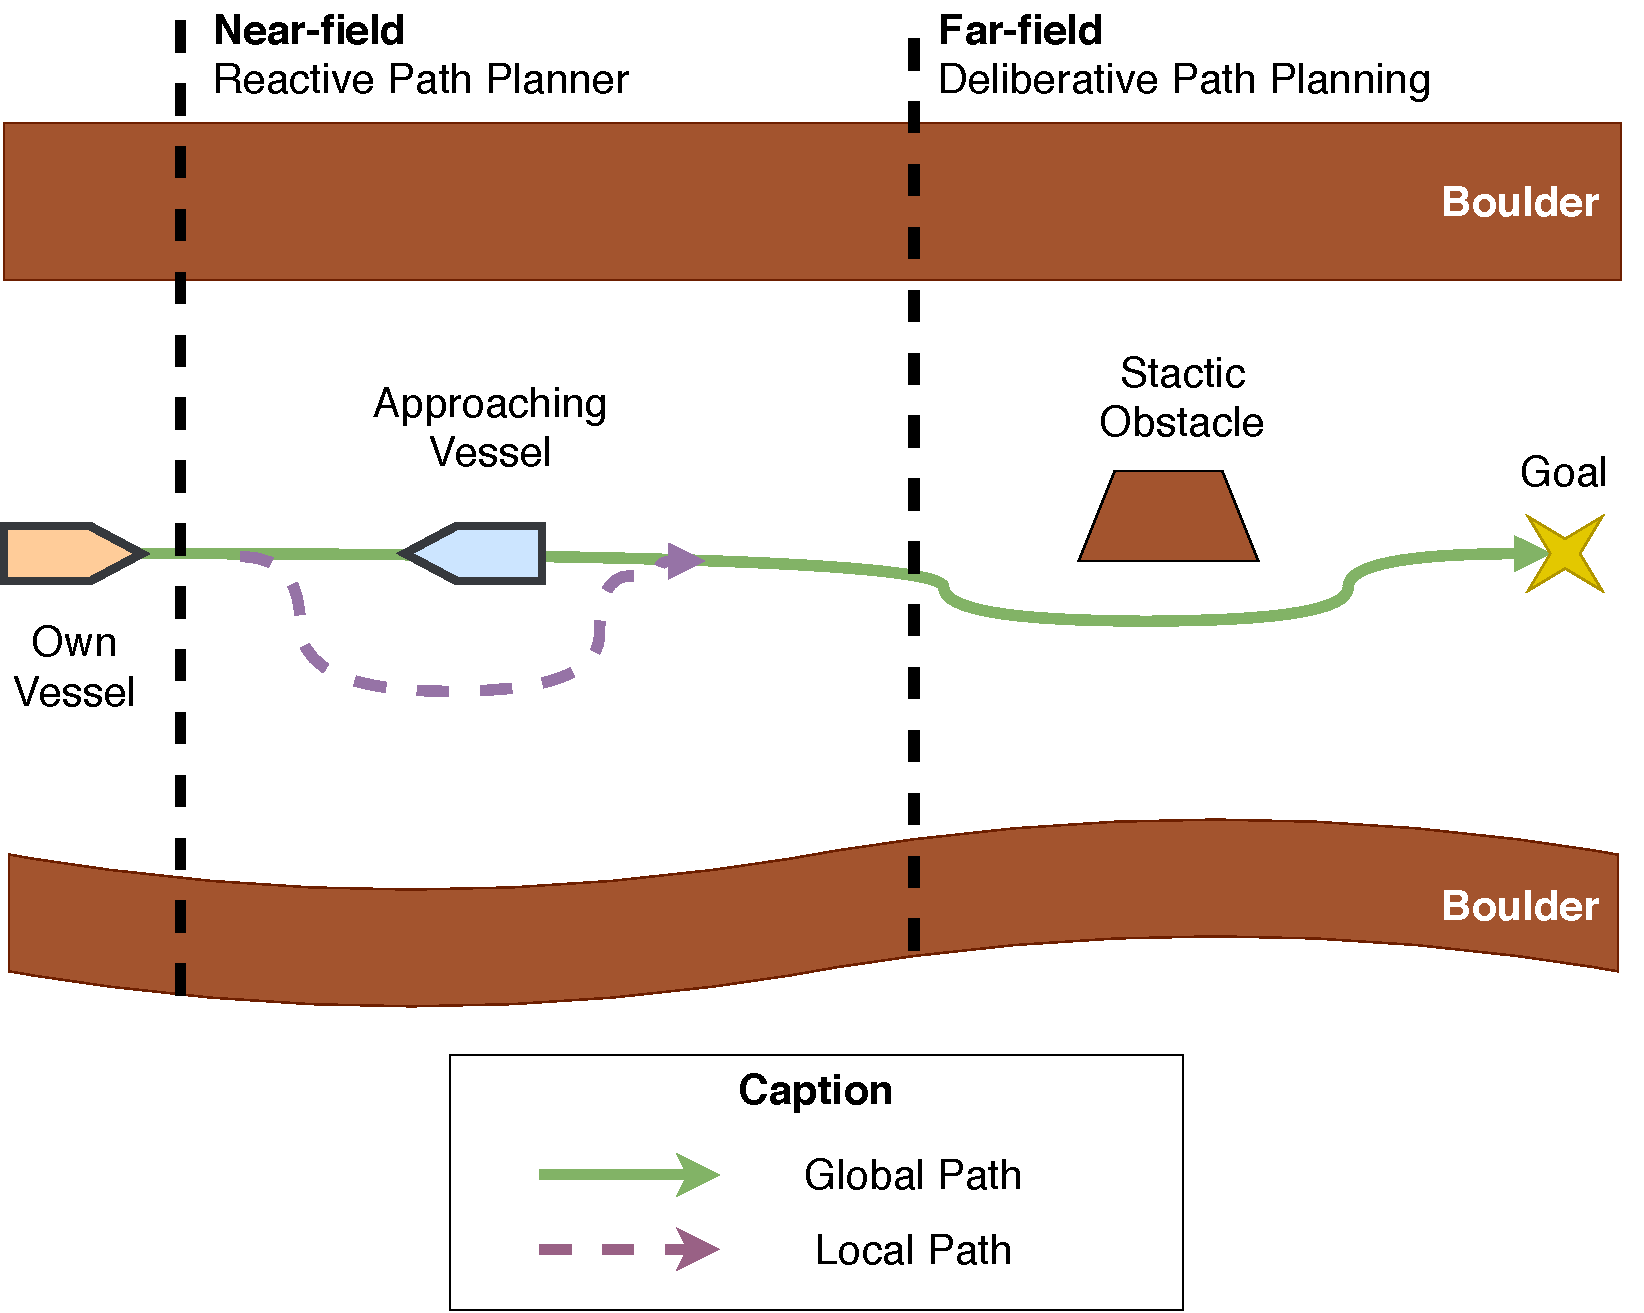
\includegraphics[scale=0.6]{figs/Chap2/GlobalLocalPath.pdf}
        \caption{Global and local paths.}
        \label{fig:chap2_globallocalpath}
    \end{figure}

    %%%%%%%%%%%%%%%%%%
    % Grammarly: 100/100
    %%%%%%%%%%%%%%%%%%
    In general, static information about the environment, such as islands, and coasts, are extracted from nautical charts, topography charts, and offline available maps. While dynamic information about the environment, such as unknown static obstacles and other vessels, is acquired in run-time by the navigation system. Also, the guidance system depends on a world representation (i.e., cost maps) for running its main component, the path planner.

    \subsection{Navigation System}
    
    %%%%%%%%%%%%%%%%%%
    %
    %%% Navigation   
    %
    %%% Grammarly: 99/100
    %%%%%%%%%%%%%%%%%%
    The navigation system is responsible for the determination of the current state of the \ac{USV} (e.g., position, velocity, orientation, and acceleration) and environment perception (e.g., static and dynamic obstacles, other vessels, wind speed, and water current). For \ac{USV}'s state estimation, the navigation system can use GPS, \ac{IMU}\footnote{For more information read https://en.wikipedia.org/wiki/Inertial\_measurement\_unit}, and compasses. Regarding environment perception, static information about the environment is extracted from nautical charts and topographic maps. While, dynamic information about the environment is acquired in real-time sensing by the navigation system through the usage of cameras, \ac{LIDAR}\footnote{For more information read https://en.wikipedia.org/wiki/Lidar}, radar, and \ac{AIS}. \ac{AIS} allows automated message exchange between vessels, facilitating the identification of location, velocity, course, path, dimension, and type of \acp{AV}.
    
    \subsection{Control System}
    %%%%%%%%%%%%%%%%%%
    %
    %%% Control
    %
    %%% Grammarly: 100/100
    %%%%%%%%%%%%%%%%%%
    The control system is responsible for the generation of actuation commands that change the \ac{USV}'s state. For an airboat (as shown in Figure \ref{fig:chap2_airboat}), for example, the control system will generate commands to change the rotation and gain of the fan. While for a differential boat (as shown in Figure \ref{fig:chap2_diffboat}), the control system will generate a gain command for each thruster. The control system determines actuation commands, considering the trajectory generated by the guidance system.
    
    \begin{figure}[H]
    \centering
    
        \begin{subfigure}[b]{0.44\textwidth}
            \centering
            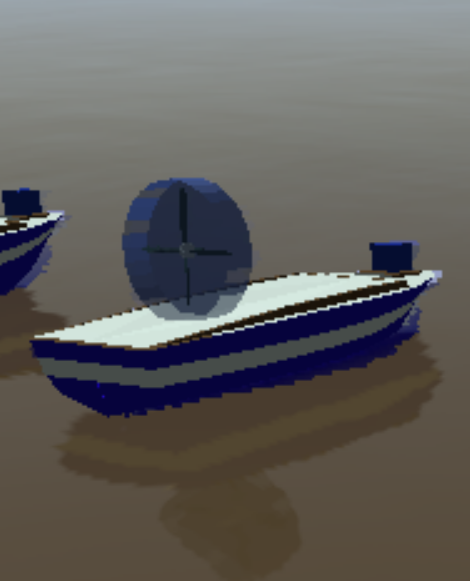
\includegraphics[scale=0.44]{figs/Chap2/airboat.png}
            \caption{Airboat with fan}
            \label{fig:chap2_airboat}
        \end{subfigure}
        \hfill
        \begin{subfigure}[b]{0.52\textwidth}
            \centering
            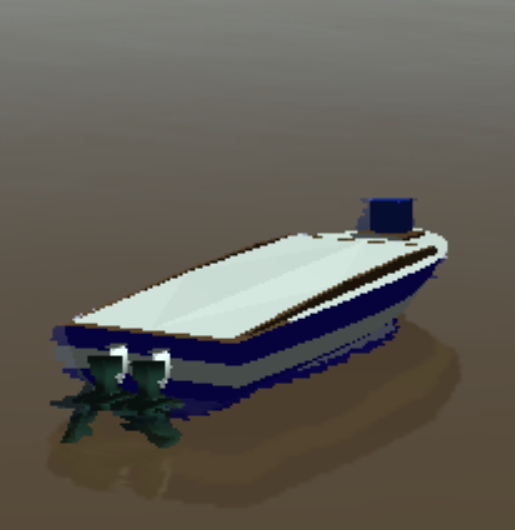
\includegraphics[scale=0.48]{figs/Chap2/diffboat2.png}
            \caption{Differential boat with two thruster}
            \label{fig:chap2_diffboat}
        \end{subfigure}
    
    \caption{Example of vessels and different propellers. Both vessels are simulated versions of Platypus~\cite{PlatypusLLC} boats we have in our laboratory.}
    \label{fig:boats}
    \end{figure}

\section{COLREGS}
\label{sec:colregs}

    %%%%%%%%%%%%%%%%%%
    %%% Grammarly: ??/100
    %%%%%%%%%%%%%%%%%%
    \ac{COLREGS}\cite{COLREGS} stands for "International Regulation for Preventing Collisions at Sea, 1972", sometimes cited as "COLlision REGulations at Sea" or "Convention on the International Regulations for Preventing Collisions at Sea" - in this work we adopted the latter. The definitions declared on the \ac{COLREGS} are controlled, updated, and of responsibility of the \ac{IMO}. Briefly, the \ac{COLREGS} defines the rules that must be followed by vessels upon waters to avoid collisions when encountering another vessel. 
    The \ac{COLREGS} are adopted by the United Nations as a global convention and must be respected by every country.
    
    %%%%%%%%%%%%%%%%%%
    %%% Grammarly: 99/100
    %%%%%%%%%%%%%%%%%%
    \ac{COLREGS} rules were not defined considering autonomous systems such as \ac{USV}s. They were written to be interpreted by well-experienced sailors and imply the usage of their experience and common sense. There are gaps to be filled and subjective or ambiguous definitions to be addressed, making the development of a \ac{COLREGS}-compliant \ac{USV} guidance system challenging.

    %%%%%%%%%%%%%%%%%%
    %%% Grammarly: 100/100
    %%%%%%%%%%%%%%%%%%
    Below we describe the four main encounters presented in \ac{COLREGS} (illustrated in Figure \ref{fig:chap2_encounters}), head-on, crossing from the right, crossing from the left, and overtaking.
    
    \begin{itemize}
        \item Head-On: In this situation both vessels should avoid collision going to their starboard side.
        \item Crossing from the right and crossing from the left: In this scenario, the \ac{COLREGS} defines different responsibilities for each vessel. The vessel that has the other vessel in its starboard side must give way and is responsible for collision avoidance. The vessel that has the other vessel in its port side must keep its course without significant changes. In a critical situation, where the give-way vessel seems not able to avoid the collision, the keep vessel should act to avoid.
        \item Overtake: In this scenario the vessel overtaking another, can freely decide which side to go and must avoid generating another crossing situation.
    \end{itemize}
    
    \begin{figure}[H]
        \centering
        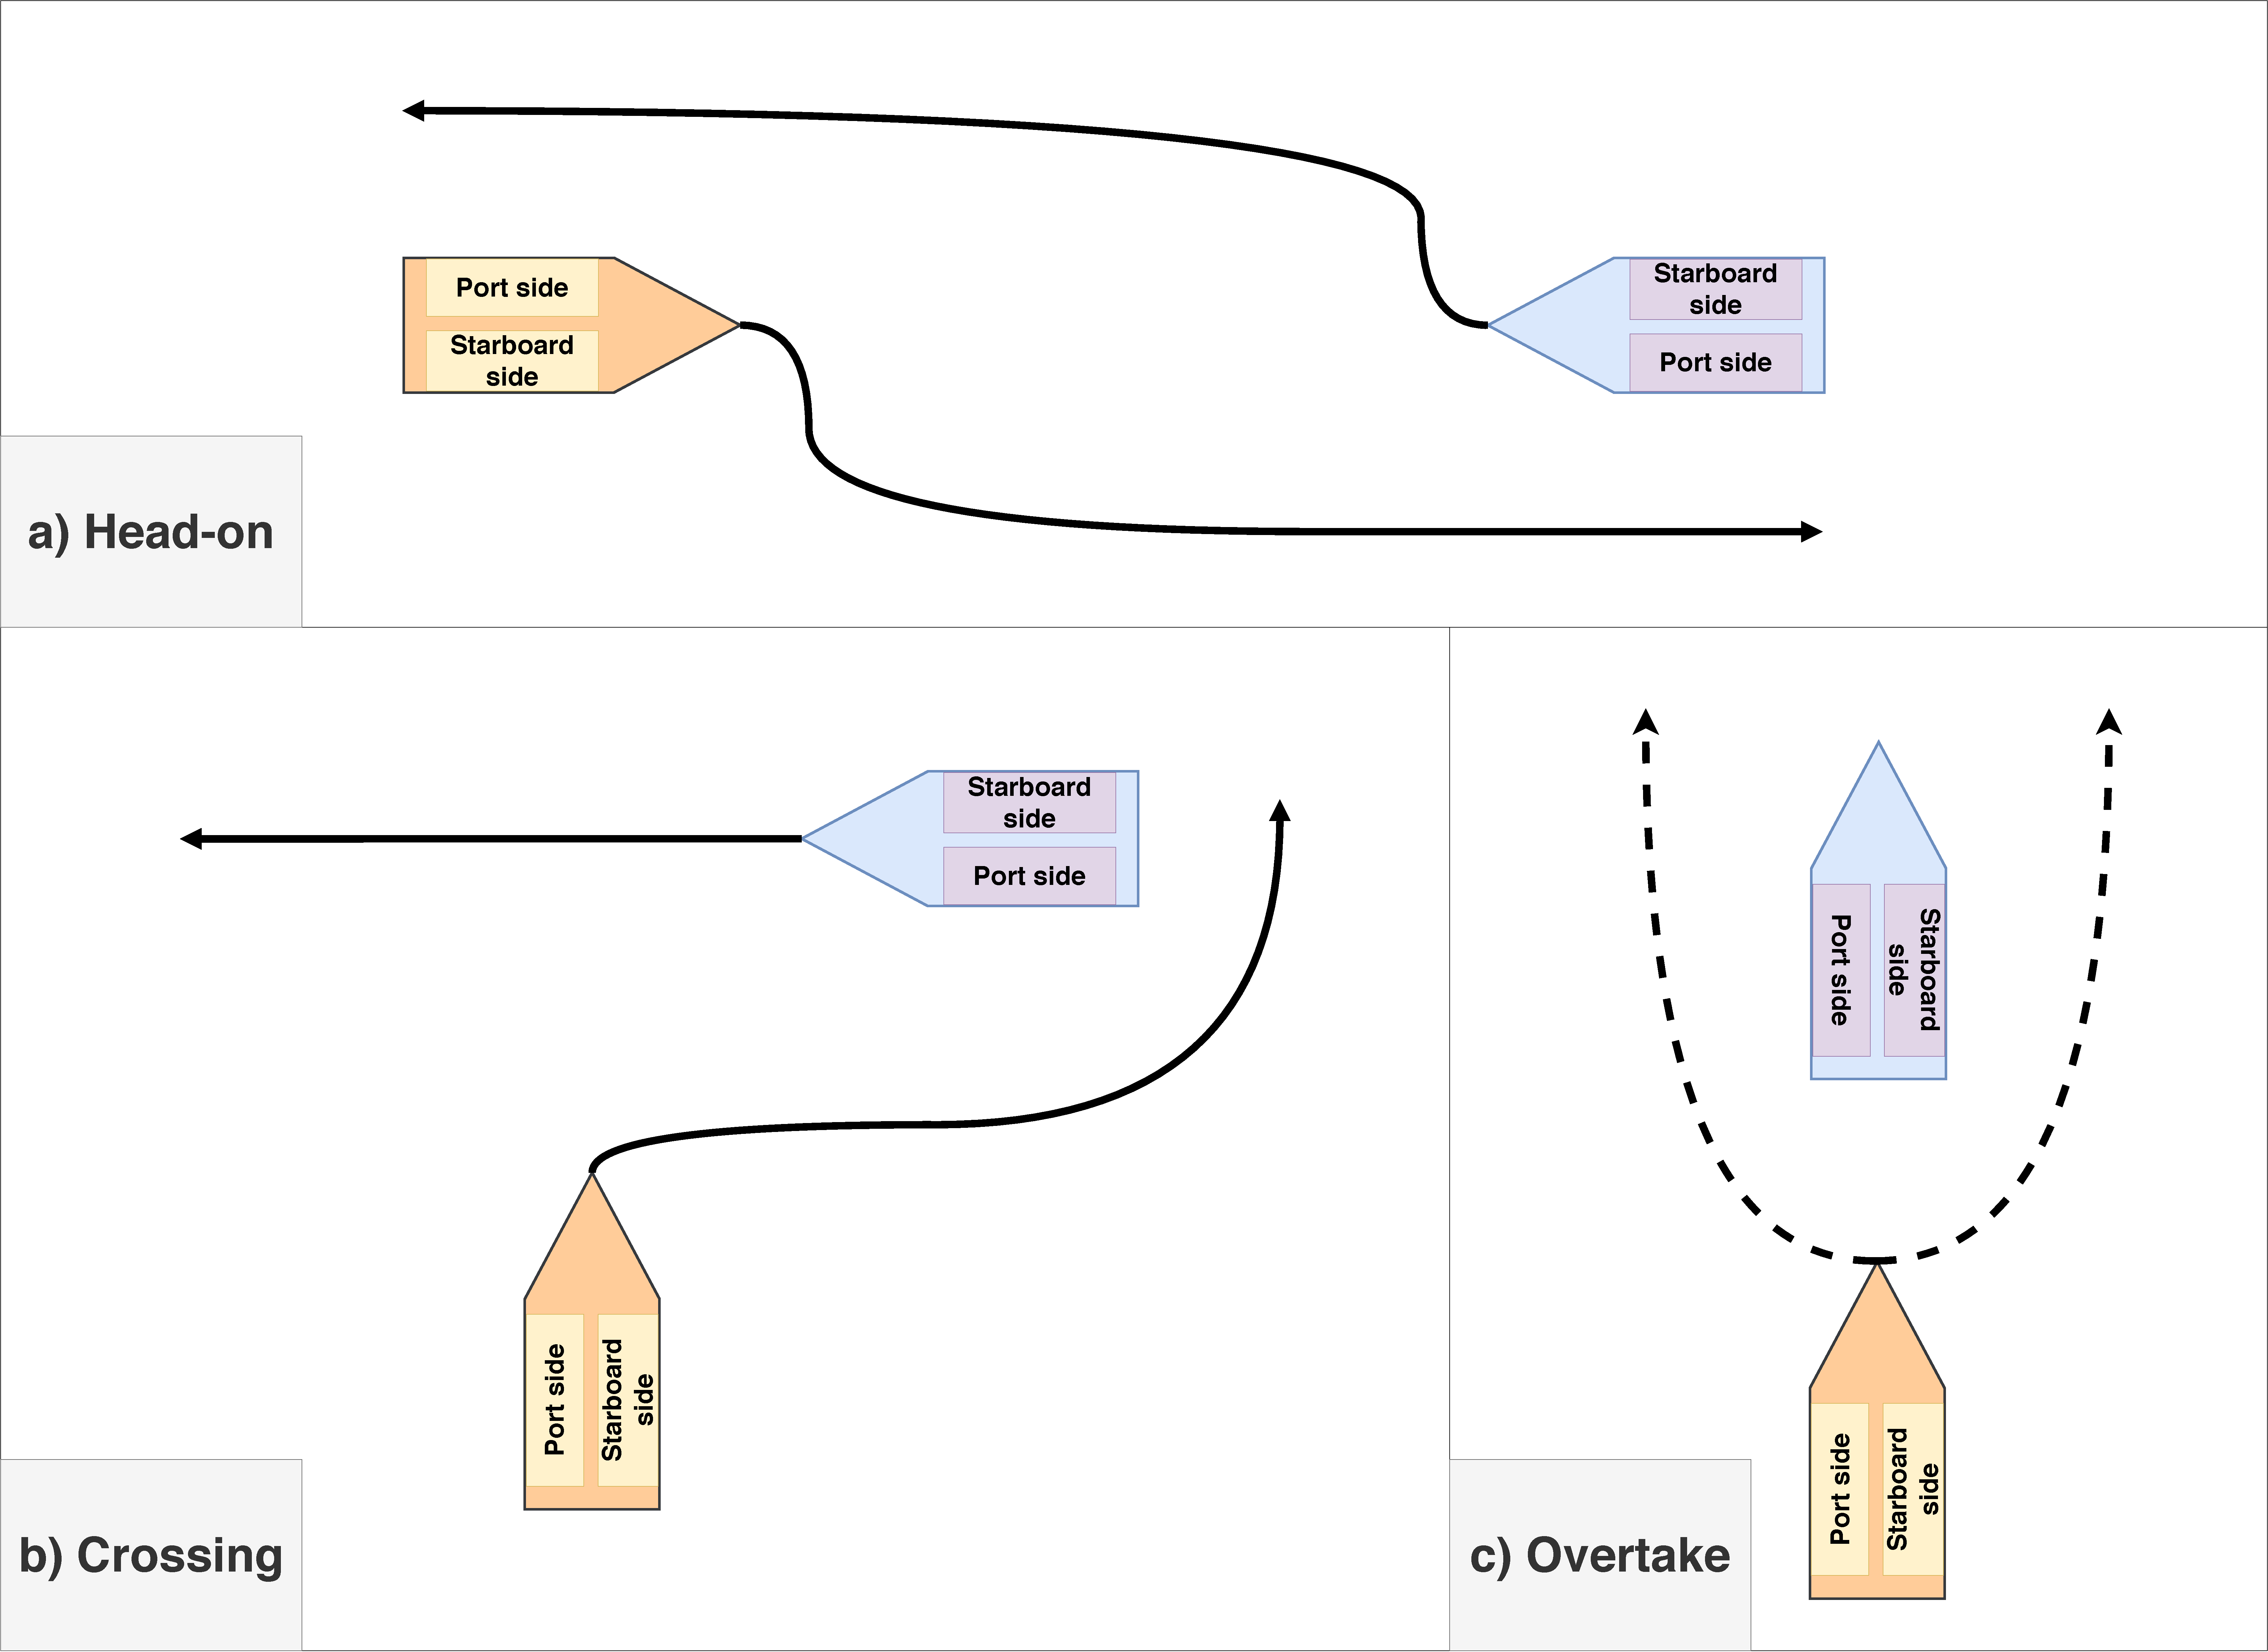
\includegraphics[scale=0.125]{figs/Chap2/Encounters.pdf}
        \caption{Possible encounters between two vessels discussed in the \ac{COLREGS}. Arrows indicate the behavior that must be performed by the vessels. In c) there are two possible paths for the orange vessel. }
        \label{fig:chap2_encounters}
    \end{figure}